 %% ****** Start of file apstemplate.tex ****** %
%%
%%
%%   This file is part of the APS files in the REVTeX 4.2 distribution.
%%   Version 4.2a of REVTeX, January, 2015
%%
%%
%%   Copyright (c) 2015 The American Physical Society.
%%
%%   See the REVTeX 4 README file for restrictions and more information.
%%
%
% This is a template for producing manuscripts for use with REVTEX 4.2
% Copy this file to another name and then work on that file.
% That way, you always have this original template file to use.
%
% Group addresses by affiliation; use superscriptaddress for long
% author lists, or if there are many overlapping affiliations.
% For Phys. Rev. appearance, change preprint to twocolumn.
% Choose pra, prb, prc, prd, pre, prl, prstab, prstper, or rmp for journal
%  Add 'draft' option to mark overfull boxes with black boxes
%  Add 'showkeys' option to make keywords appear
\documentclass[aps,prl,preprint,groupedaddress]{revtex4-2}
\usepackage[UTF8]{ctex}
\usepackage{graphicx}
\usepackage{float}
%\documentclass[aps,prl,preprint,superscriptaddress]{revtex4-2}
%\documentclass[aps,prl,reprint,groupedaddress]{revtex4-2}

% You should use BibTeX and apsrev.bst for references
% Choosing a journal automatically selects the correct APS
% BibTeX style file (bst file), so only uncomment the line
% below if necessary.
%\bibliographystyle{apsrev4-2}

\begin{document}
\renewcommand{\thesection}{\Roman{section}}
% Use the \preprint command to place your local institutional report
% number in the upper righthand corner of the title page in preprint mode.
% Multiple \preprint commands are allowed.
% Use the 'preprintnumbers' class option to override journal defaults
% to display numbers if necessary
%\preprint{}

%Title of paper
\title{相对论效应实验报告}

% repeat the \author .. \affiliation  etc. as needed
% \email, \thanks, \homepage, \altaffiliation all apply to the current
% author. Explanatory text should go in the []'s, actual e-mail
% address or url should go in the {}'s for \email and \homepage.
% Please use the appropriate macro foreach each type of information

% \affiliation command applies to all authors since the last
% \affiliation command. The \affiliation command should follow the
% other information
% \affiliation can be followed by \email, \homepage, \thanks as well.
\author{林照翔}
%\email[]{Your e-mail address}
%\homepage[]{Your web page}
%\thanks{}
%\altaffiliation{}
\affiliation{2022级理论物理2班\\学号:320220935801\\组号:38}

%Collaboration name if desired (requires use of superscriptaddress
%option in \documentclass). \noaffiliation is required (may also be
%used with the \author command).
%\collaboration can be followed by \email, \homepage, \thanks as well.
%\collaboration{}
%\noaffiliation

\date{\today}

\begin{abstract}
% insert abstract here
本实验通过测量高速运动电子的动量和动能来验证狭义相对论的动量和动能关系。通过本次实验可以简单了解半聚焦磁谱仪的原理与应用,掌握 $\gamma-\beta $ 闪烁谱仪以及多道脉冲器的应用并通过数据处理及计算机软件绘图提高实验研究的基本能力。

\end{abstract}

% insert suggested keywords - APS authors don't need to do this
%\keywords{}

%\maketitle must follow title, authors, abstract, and keywords
\maketitle

% body of paper here - Use proper section commands
% References should be done using the \cite, \ref, and \label commands
\section{I. 引言}
% Put \label in argument of \section for cross-referencing
%\section{\label{}}
\subsection{A. 相对论效应实验原理}

\subsubsection{1. 经典力学中动能和动量的关系}

经典力学中,电子动能 $E_k$ 和动量 $p$ 的关系为:

$$
E_k = \frac{p^2}{2m_0}
$$

其中,$m_0$ 是电子的静止质量。

\subsubsection{2. 狭义相对论中能量和动量的关系}

在狭义相对论中,爱因斯坦质能方程给出:

$$
E = m c^2
$$

其中,$E$ 是运动电子的总能量,$m $ 是运动电子的动质量,$c $ 是光速。

$$
m = \frac{m_0}{\sqrt{1-v^2/c^2}}
$$

其中,$v$ 是电子的速度。

当电子静止时,静止能量为:

$$
E_0 = m_0 c^2
$$

狭义相对论中电子的能量和动量的关系:

$$
E^2-p^2c^2
=m^2 c^4-m^2v^2c^2
=m^2c^2(c^2-v^2)
=\frac{m_0^2}{1-v^2/c^2}c^2(c^2-v^2)
=m_0^2c^4
$$

电子的动能是电子的总能量与静止能量之差:

$$
E_k
=E-E_0
=\sqrt{(p^2c^2)+\left(m_0c^2\right)^2} - m_0c^2
$$

这就是狭义相对论中动能与动量的关系。

\section{II. 实验方法}

\subsection{A. 半圆形磁谱仪}

$\beta $ 源射出的高速 $\beta$ 粒子经准直后垂直入射一竖直方向的均匀磁场,粒子受与运动方向垂直的洛伦兹力而作圆周运动。运动方程为:

$$
evB = \frac{mv^2}{R}
$$

因此:

$$
v = \frac{eBR}{m}
$$

$$
p = mv = eBR
$$

其中,$R$ 为圆形轨道的半径,为源与探测器间距的一半:

$$
R = \frac{1}{2}(x-x_0)
$$

其中,$x_0$ 是源的位置,$x$ 是探测器的位置。

\subsection{B. 能量定标}

闪烁探测器采用多道分析器,$\beta$ 粒子的动能 $E_k$ 与道数 $\mathrm{CH}$ 成正比。本实验采用 $137\mathrm{Cs} $ 标准源进行能量定标。动能与道数的关系为:

$$
E_k = a+b\times \mathrm{CH}
$$

\begin{table}[htbp] % [htbp] 表示表格的浮动位置
	\centering % 使表格居中
	\caption{能量定标} % 表格标题
	\begin{tabular}{|c|c|c|c|} % 定义表格和对齐方式
	\hline % 顶部线条
	能量($\mathrm{MeV}$) & 0.184 &0.662 \\ % 第一行内容
	\hline % 水平线条
	道数 &92 &727 \\ % 第二行内容
	\hline % 底部线条
	\end{tabular}
\end{table}

从中可以得到:

$$
a = 0.115\mathrm{MeV} ,~~b = 7.53\times 10^{-4} \mathrm{MeV}
$$

\section{III. 结果与讨论}

\subsection{A. 实验结果和数据处理}

放射源位置 $x_0=9.50\mathrm{cm}$,磁场强度 $B=740\mathrm{G}$

\begin{table}[H] % [htbp] 表示表格的浮动位置
	\centering % 使表格居中
	\caption{探测器位置与道数关系} % 表格标题
	\begin{tabular}{|c|c|c|c|c|c|c|} % 定义表格和对齐方式
	\hline % 顶部线条
	探测器位置 $x$ ($\mathrm{cm}$) &34.90  &32.40 &30.00 &27.50 &24.00 &22.00  \\ % 第一行内容
	\hline % 水平线条
	道数 $\mathrm{CH }$ &995 &809 &581 &435 &335 &237\\ % 第二行内容
	\hline % 底部线条
	\end{tabular}
\end{table}

根据 $p=eB(x-x_0)/2,E_k=a+b\times\mathrm{CH}$ 可得:

\begin{table}[H] % [htbp] 表示表格的 浮动位置
	\centering % 使表格居中
	\caption{动能与动量关系} % 表格标题
	\begin{tabular}{|c|c|c|c|c|c|c|} % 定义表格和对齐方式
	\hline % 顶部线条
	$pc$ ($\mathrm{MeV}$) &2.8149  &2.5419 &2.2755 &1.9980 &1.6095 &1.3875  \\ % 第一行内容
	\hline % 水平线条
	动能 $E_k$ ($\mathrm{MeV }$) &0.8642 &0.7241 &0.5525 &0.4426 &0.3673 &0.2935\\ % 第二行内容
	\hline % 底部线条
	\end{tabular}
\end{table}

采用 $pc $ 而非 $p$ 作为横坐标,是为了使动能 $E_k$ 与 $pc$ 的数值在 数量级上相差不大。且  $E_k$ 与 $pc$ 有相同量纲,更便于分析二者关系。

\begin{figure}[H]
    \centering
    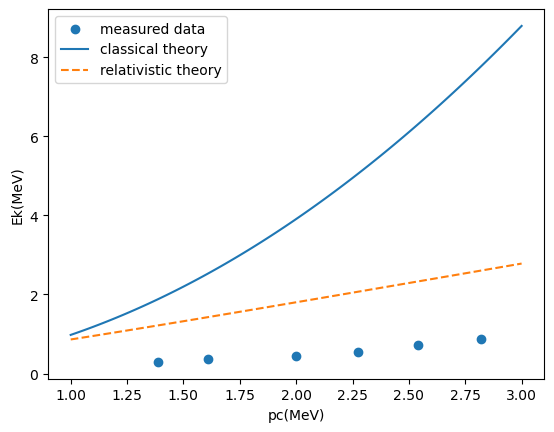
\includegraphics[width=0.8\textwidth]{img/1.png}
    \caption{Ek与pc关系图}
    \label{1}
\end{figure}

\section{IV. 结论}

本实验通过测量高速运动电子的动量和动能来验证狭义相对论的动量和动能关系。将所测数据点分别与经典的动量-动能关系和相对论的动量-动能关系的线型进行对比,验证了高速运动的电子的动量-动能关系服从相对论的动量-动能关系。

% If in two-column mode, this environment will change to single-column
% format so that long equations can be displayed. Use
% sparingly.
%\begin{widetext}
% put long equation here
%\end{widetext}

% figures should be put into the text as floats.
% Use the graphics or graphicx packages (distributed with LaTeX2e)
% and the \includegraphics macro defined in those packages.
% See the LaTeX Graphics Companion by Michel Goosens, Sebastian Rahtz,
% and Frank Mittelbach for instance.
%
% Here is an example of the general form of a figure:
% Fill in the caption in the braces of the \caption{} command. Put the label
% that you will use with \ref{} command in the braces of the \label{} command.
% Use the figure* environment if the figure should span across the
% entire page. There is no need to do explicit centering.

% \begin{figure}
% \includegraphics{}%
% \caption{\label{}}
% \end{figure}

% Surround figure environment with turnpage environment for landscape
% figure
% \begin{turnpage}
% \begin{figure}
% \includegraphics{}%
% \caption{\label{}}
% \end{figure}
% \end{turnpage}

% tables should appear as floats within the text
%
% Here is an example of the general form of a table:
% Fill in the caption in the braces of the \caption{} command. Put the label
% that you will use with \ref{} command in the braces of the \label{} command.
% Insert the column specifiers (l, r, c, d, etc.) in the empty braces of the
% \begin{tabular}{} command.
% The ruledtabular enviroment adds doubled rules to table and sets a
% reasonable default table settings.
% Use the table* environment to get a full-width table in two-column
% Add \usepackage{longtable} and the longtable (or longtable*}
% environment for nicely formatted long tables. Or use the the [H]
% placement option to break a long table (with less control than 
% in longtable).
% \begin{table}%[H] add [H] placement to break table across pages
% \caption{\label{}}
% \begin{ruledtabular}
% \begin{tabular}{}
% Lines of table here ending with \\
% \end{tabular}
% \end{ruledtabular}
% \end{table}

% Surround table environment with turnpage environment for landscape
% table
% \begin{turnpage}
% \begin{table}
% \caption{\label{}}
% \begin{ruledtabular}
% \begin{tabular}{}
% \end{tabular}
% \end{ruledtabular}
% \end{table}
% \end{turnpage}

% Specify following sections are appendices. Use \appendix* if there
% only one appendix.
%\appendix
%\section{}

% If you have acknowledgments, this puts in the proper section head.
%\begin{acknowledgments}
% put your acknowledgments here.
%\end{acknowledgments}

% Create the reference section using BibTeX:

\end{document}
%
% ****** End of file apstemplate.tex ******

